\documentclass{article}
\usepackage[english]{babel}
\usepackage{indentfirst}
\usepackage{tikz, pgfplots}
\usepackage{graphics}
\usepackage{amsthm}
\usepackage{amssymb}
\usepackage{amsmath}
\usepackage{verbatim}
\usepackage{mathrsfs}
\usepackage[mathcal]{euscript}
\usepackage{fancyhdr}
\usepackage{enumitem}
\usepackage{titlesec}
\usepackage{tocloft}
\usepackage[a4paper]{geometry}

\geometry{top=50pt, left=50pt, right=50pt}
\usetikzlibrary{positioning}
\usetikzlibrary{calc}





\pagestyle{fancy}
\lhead{}
\rhead{\thepage\ of \pageref{LastPage}}
\chead{}
\lfoot{}
\rfoot{}
\cfoot{}

% \renewcommand{\headrulewidth}{0pt}
% \renewcommand{\footrulewidth}{0pt}

\renewcommand\cftsecdotsep{\cftdot}
\renewcommand\cftsubsecdotsep{\cftdot}
\renewcommand\cftsecafterpnum{\vskip5pt}
\renewcommand\cftsubsecafterpnum{\vskip5pt}
\renewcommand\cftsecfont{\normalfont}
\renewcommand\cftsecpagefont{\normalfont}
\renewcommand{\cftsecleader}{\cftdotfill{\cftsecdotsep}}



\usepackage[unicode]{hyperref}
\hypersetup{
    colorlinks=true,
    citecolor=black,
    filecolor=black,
    linkcolor=black,
    urlcolor=black,
}
\usepackage[numbered]{bookmark}
\usetikzlibrary{calc}
\titleformat{\section}[block]{\Large\thesection.~}{}{0mm}{}
\titleformat{\subsection}[block]{\it\large\thesubsection.}{}{1mm}{}
% \titleformat{\subsection}[block]{\filcenter\large}{}{1mm}{}

\titlespacing*{\section}{0mm}{10mm}{10mm}
\titlespacing*{\subsection}{0mm}{10mm}{8mm}

\def\arraystretch{1.5}
\numberwithin{equation}{section}

\newtheorem{lemma}{Lemma}[section]
\newtheorem{theorem}{Theorem}[section]
\newtheorem{hypothesis}{Hypothesis}[section]

\theoremstyle{definition}
\newtheorem{definition}{Definition}[section]

\theoremstyle{remark}
\newtheorem{example}{Example}[section]
\newtheorem{remark}{Remark}[section]


\newcommand{\dsum}{\displaystyle\sum}
\newcommand{\ceil}[1]{\left\lceil #1 \right\rceil}
\newcommand{\floor}[1]{\left\lfloor #1 \right\rfloor}
\renewcommand{\mod}[1]{~\mathrm{mod}\left(#1\right)}
\renewcommand{\emptyset}{\text{\O}}


\newcommand{\quoted}[1]{\textquotedblleft#1\textquotedblright}


\def\layersep{2.5cm}



\usepackage{color}



\begin{document}
\title{Mathematics and Artificial Neural Network}
\author{Giorgi Kakulashvili}
\date{\today}
\maketitle
\thispagestyle{fancy}



\tableofcontents

\newpage


\section{Artificial Neural Network}

Suppose we have two finite sets of vectors in $X$ and $Y$
\[
    X = \left\{ \left( x_1^{j}, x_2^{j},\dots, x_n^{j} \right) : 1 \le j \le N_{x},~ x_{i}^{j} \in [0,1]  \right\}
\]
\[
    Y = \left\{ \left( y_1^{j}, y_2^{j},\dots, y_m^{j} \right) : 1 \le j \le N_{y},~ y_{i}^{j} \in [0,1] \right\}
\]
and there exists surjective mapping
\[
    f: X\to Y
\]
such that for all $x\in X$ we know corresponding $f(x)=y\in Y$, then we can construct $\hat{f}$ function, which will approximate $f$ function.

For simplicity we'll be using $X$ and $Y$ as matrices
\[
    X = \begin{bmatrix}
        x_{1}^1 & x_{1}^2 & \cdots & x_{1}^{N_x} \\
        x_{2}^1 & x_{2}^2 & \cdots & x_{2}^{N_x} \\
        \vdots & \vdots & \ddots & \vdots \\
        x_{n}^1 & x_{n}^2 & \cdots & x_{n}^{N_x} \\
    \end{bmatrix}
    ~~\textit{and}~~
    Y = \begin{bmatrix}
        y_{1}^1 & y_{1}^2 & \cdots & y_{1}^{N_y} \\
        y_{2}^1 & y_{2}^2 & \cdots & y_{2}^{N_y} \\
        \vdots & \vdots & \ddots & \vdots \\
        y_{m}^1 & y_{m}^2 & \cdots & y_{m}^{N_y} \\
    \end{bmatrix}
\]
Let $X_{j}$ and $Y_{j}$ be corresponding columns, then for all $i$, there exists $j$, such that
\[
    f(X_{i}) = Y_{j}
\]

For constructing $\hat{f}$ function we are using \textit{Neural Network}, which is commonly visualized like

\begin{center}
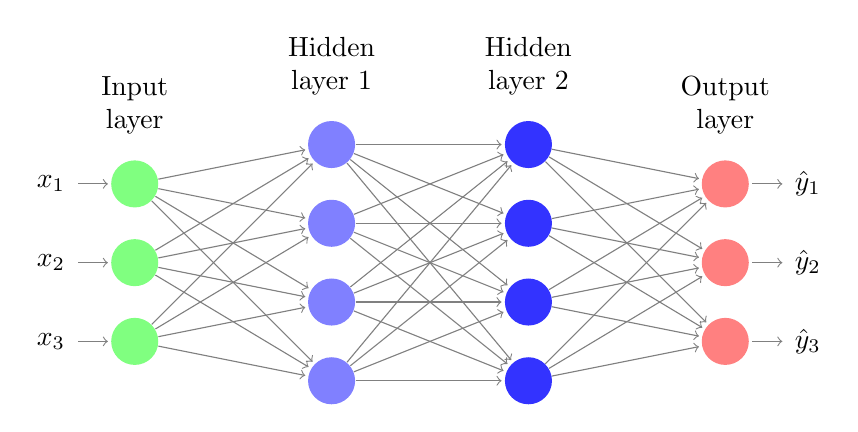
\begin{tikzpicture}[shorten >=1pt,->,draw=black!50, node distance=\layersep]
        \tikzstyle{every pin edge}=[<-,shorten <=1pt]
        \tikzstyle{neuron}=[circle,fill=black!25,minimum size=17pt,inner sep=0pt]
        \tikzstyle{input neuron}=[neuron, fill=green!50];
        \tikzstyle{output neuron}=[neuron, fill=red!50];
        \tikzstyle{hidden neuron}=[neuron, fill=blue!50];
        \tikzstyle{hidden2 neuron}=[neuron, fill=blue!80];
        \tikzstyle{annot} = [text width=4em, text centered]

        % Draw the input layer nodes
        \node[input neuron, pin=left:$x_1$] (I-1) at (0,-1) {};
        \node[input neuron, pin=left:$x_2$] (I-2) at (0,-2) {};
        \node[input neuron, pin=left:$x_3$] (I-3) at (0,-3) {};

        % Draw the hidden layer nodes
        \foreach \name / \y in {1,...,4}
            \path[yshift=0.5cm]
                node[hidden neuron] (H-\name) at (\layersep,-\y cm) {};

        \foreach \name / \y in {1,...,4}
            \path[yshift=0.5cm]
                    node[hidden2 neuron] (H2-\name) at (2*\layersep,-\y cm) {};

        \foreach \name / \y in {1,...,3}
            \path
                node[output neuron, pin={[pin edge={->}]right:$\hat{y}_\name$}] (O-\name) at (3*\layersep,-\y cm) {};


        % Connect every node in the input layer with every node in the
        \foreach \source in {1,...,3}
            \foreach \dest in {1,...,4}
                \path (I-\source) edge (H-\dest);

        \foreach \source in {1,...,4}
            \foreach \dest in {1,...,4}
                \path (H-\source) edge (H2-\dest);

        \foreach \source in {1,...,4}
            \foreach \dest in {1,...,3}
                    \path (H2-\source) edge (O-\dest);

        % Annotate the layers
        \node[annot,above of=I-1, node distance=1cm] (il) {Input layer};
        \node[annot,above of=H-1, node distance=1cm] (hl) {Hidden layer 1};
        \node[annot,above of=H2-1, node distance=1cm] (h2) {Hidden layer 2};
        \node[annot,above of=O-1, node distance=1cm] (o1) {Output layer};

\end{tikzpicture}
\end{center}

\noindent
Here first and last layers are inputs and output and number of neurons depend on vector size, while \textit{hidden layers} are chosen. Suppose we have $L+1$ layers, with $n_{l}$ neurons in $l$ layer.

For given $X_i$ vector calculation of $\hat{f} \left( X_i \right)$ is \textit{forward propagation}




\subsection{Forward Propagation}



All nodes are connected with each other. Each connection has weight and each neuron, expect inputs, have biases. To get values of neurons in layer $l+1$, we need to do following opertaions
\[
    z^{(l)} =
    \begin{bmatrix}
        z_{1}^{(l)} \\
        z_{2}^{(l)} \\
        \vdots \\
        z_{n_{l}}^{(l)}
    \end{bmatrix} =
    \begin{bmatrix}
        w_{11}^{(l)} & w_{12}^{(l)} & \cdots & w_{1n_{l-1}}^{(l)} \\
        w_{21}^{(l)} & w_{22}^{(l)} & \cdots & w_{2n_{l-1}}^{(l)} \\
        \vdots & \vdots & \ddots & \vdots \\
        w_{n_{l}1}^{(l)} & w_{n_{l}2}^{(l)} & \cdots & w_{n_{l}n_{l-1}}^{(l)} \\
    \end{bmatrix} \times
    \begin{bmatrix}
        a_{1}^{(l-1)} \\
        a_{2}^{(l-1)} \\
        \vdots \\
        a_{n_{l-1}}^{(l-1)}
    \end{bmatrix} +
    \begin{bmatrix}
        b_{1}^{(l)} \\
        b_{2}^{(l)} \\
        \vdots \\
        b_{n_{l}}^{(l)}
    \end{bmatrix}
    = w^{(l)} a^{(l-1)} + b^{(l)}
\]

\noindent
and by activation function $\sigma$, we have

\[
    a^{(l)} =
    \begin{bmatrix}
       a_{1}^{(l)} \\[5pt]
       a_{2}^{(l)} \\[5pt]
        \vdots \\[5pt]
       a_{n_{l}}^{(l)}
    \end{bmatrix} =
    \begin{bmatrix}
       \sigma\left( z_{1}^{(l)} \right)\\[5pt]
       \sigma\left( z_{2}^{(l)} \right)\\[5pt]
        \vdots \\[5pt]
       \sigma\left( z_{n_{l}}^{(l)} \right)
    \end{bmatrix}
    = \sigma \left( z^{(l)} \right), \quad
    a^{(0)} = X = \begin{bmatrix}
       x_{1} \\[5pt]
       x_{2} \\[5pt]
        \vdots \\[5pt]
       x_{n_{0}}
    \end{bmatrix}, \quad a^{(L)} = \hat{Y} = \begin{bmatrix}
       \hat{y}_{1} \\[5pt]
       \hat{y}_{2} \\[5pt]
        \vdots \\[5pt]
       \hat{y}_{n_{L}}
    \end{bmatrix}
\]

\noindent
Here we take activation function
\[
    \sigma \left( x \right) = \frac{1}{1+e^{-x}}
\]
which maps $\mathbb{R}$ to $(0,1)$, and its derivitive is
\[
    \sigma' \left( x \right) = \sigma \left( x \right)
    \left( 1 - \sigma \left( x \right) \right)
\]




\subsection{Backward Propagation}

As we can see from \textit{Forward Propagation}, artificial neural network is continuous multidimensional function
\[
    f: X \to Y, \quad \hat{f}: X \to \hat{Y}, \quad \hat{f} \approx f
\]
Output of the function depends on weights and biases, so we need to adjust them. Since our function is divided into layers, we have cost function on each of them
\[
    C_{0} = \frac{1}{2} \left\| \hat{y} - y \right\|^2 = \frac{1}{2} \sum_{j} \left( \hat{y}_{j} - y_{j} \right)^2, \quad
    C_{k} = \frac{1}{2} \left\| a^{(L-k)} - \tilde{a}^{(L-k)} \right\|^2 =
    \frac{1}{2} \left\| \delta^{(L-k)} \right\|^2, \quad
    C =  \sum_{k=0}^{L-1} C_{k}
\]
$C$ function depends on $w_{jk}^{(l)}$ and $b_{j}^{(l)}$ parameters and by tilde symbol we denote that it is corrected version. Our goal is to minimize cost function, and for this we use \textit{gradient descent} method. For this we need to calculate partial derivatives.

In output layer we have following equations
\begin{align}
a_{j}^{(L)} &= \sigma \left( z_{j}^{(L)} \right) \\
z_{j}^{(L)} &= \sum_{k=1}^{n_{L-1}} w_{jk}^{(L)} a_{k}^{(L-1)} + b_{j}^{(L)} \\
C_{0} &= \frac{1}{2} \sum_{j=1}^{n_{L}} \left( a_{j}^{(L)} - y_{j} \right)^2
\end{align}
And by chain rule we get following
\[
    \frac{\partial C_{0}}{\partial w_{jk}^{(L)}} =
    \frac{\partial z_{j}^{(L)}}{\partial w_{jk}^{(L)}}
    \frac{\partial a_{j}^{(L)}}{\partial z_{j}^{(L)}}
    \frac{\partial C_{0}}{\partial a_{j}^{(L)}} =
    a_{k}^{(L-1)} \sigma' \left( z_{j}^{(L)} \right)
    \left( a_{j}^{(L)} - y_{j} \right) =
    a_{k}^{(L-1)} \sigma' \left( z_{j}^{(L)} \right)\delta_{j}^{(L)}
\]
\[
    \frac{\partial C_{0}}{\partial b_{j}^{(L)}} =
    \frac{\partial z_{j}^{(L)}}{\partial b_{j}^{(L)}}
    \frac{\partial a_{j}^{(L)}}{\partial z_{j}^{(L)}}
    \frac{\partial C_{0}}{\partial a_{j}^{(L)}} =
    \sigma' \left( z_{j}^{(L)} \right)\delta_{j}^{(L)}
\]
\[
    \frac{\partial C_{0}}{\partial a_{k}^{(L-1)}} =
    \sum_{j=1}^{n_{L}}
    \frac{\partial z_{j}^{(L)}}{\partial a_{k}^{(L-1)}}
    \frac{\partial a_{j}^{(L)}}{\partial z_{j}^{(L)}}
    \frac{\partial C_{0}}{\partial a_{j}^{(L)}} =
    \sum_{j=1}^{n_{L}}
    w_{jk}^{(L)} \sigma' \left( z_{j}^{(L)} \right) \delta_{j}^{(L)}
\]
If we rewrite it in matrix form, we get
\[
    \frac{\partial C_{0}}{\partial w^{(L)}} =
    \left(  \frac{\partial C_{0}}{\partial w_{jk}^{(L)}} \right)_{n_{L}\times n_{L-1}}=
    \left( a_{k}^{(L-1)} \sigma' \left( z_{j}^{(L)} \right)\delta_{j}^{(L)}  \right)_{n_{L}\times n_{L-1}}
    = \sigma' \left( z^{(L)} \right)\delta^{(L)} \left(  a^{(L-1)} \right) ^T
\]\[
    \frac{\partial C_{0}}{\partial b^{(L)}} =
    \left(  \frac{\partial C_{0}}{\partial b_{j}^{(L)}} \right)_{n_{L}\times 1} =
    \sigma' \left( z^{(L)} \right)\delta^{(L)}
\]\[
    \frac{\partial C_{0}}{\partial a^{(L-1)}} =
    \left(  \frac{\partial C_{0}}{\partial a_{k}^{(L-1)}} \right)_{n_{L-1}\times 1}=
    \left(  \sum_{j=1}^{n_{L}} w_{jk}^{(L)} \sigma' \left( z_{j}^{(L)} \right) \delta_{j}^{(L)} \right)_{n_{L-1}\times 1}=
    \left(  w^{(L)} \right)^T \sigma' \left( z^{(L)} \right)\delta^{(L)}
\]
where $\sigma'(z^{(L)})$ is diagonal matrix
\[
    \sigma'(z^{(l)}) = \begin{bmatrix}
        \sigma' \left( z_1^{(l)} \right)  & 0 & \cdots & 0 \\
        0 & \sigma' \left( z_2^{(l)} \right) & \cdots & 0 \\
        \vdots & \vdots & \ddots & \vdots \\
        0 & 0 & \cdots &\sigma' \left( z_{n_{l}}^{(l)} \right) \\
    \end{bmatrix}
\]
Now we have formulas for backward propagation, and since $\tilde{a}^{(L)}=Y$ and $a^{(L)}=\hat{Y}$, we can simply generalize is for $l$ layer
\begin{align}
\delta^{(l)} &= a^{(l)} - \tilde{a}^{(l)}\\[5pt]
\frac{\partial C_{L-l}}{\partial w^{(l)}} &= \sigma' \left( z^{(l)} \right)\delta^{(l)} \left(  a^{(l-1)} \right) ^T \\[5pt]
\frac{\partial C_{L-l}}{\partial b^{(l)}} &= \sigma' \left( z^{(l)} \right)\delta^{(l)} \\[5pt]
\frac{\partial C_{L-l}}{\partial a^{(l-1)}} &= \left(  w^{(l)} \right)^T \sigma' \left( z^{(l)} \right)\delta^{(l)}
\end{align}

\noindent
From here we can choose algorithms for finding local minimum. Let's take small $0<\gamma\le1$ and write
\begin{align*}
\tilde{w}^{(l)} &= w^{(l)} - \gamma \frac{\partial C_{L-l}}{\partial w^{(l)}}\\[5pt]
\tilde{b}^{(l)} &= b^{(l)} - \gamma \frac{\partial C_{L-l}}{\partial b^{(l)}}\\[5pt]
\tilde{a}^{(l-1)} &= a^{(l-1)} - \gamma \frac{\partial C_{L-l}}{\partial a^{(l-1)}}
\end{align*}

\noindent
So, we have $a^{(0)} = X$, $\delta^{(L)} = a^{(L)} - Y$ and

\begin{align*}
\delta b^{(l)} &= \gamma \sigma' \left( z^{(l)} \right)\delta^{(l)}\\[5pt]
\delta^{(l-1)} &= \left(  w^{(l)} \right)^T \delta b^{(l)}\\[5pt]
\tilde{b}^{(l)} &= b^{(l)} - \delta b^{(l)} \\[5pt]
\tilde{w}^{(l)} &= w^{(l)} - \delta b^{(l)}  \left(  a^{(l-1)} \right)^T\\[5pt]
\end{align*}























\end{document}



\begin{comment}


\newpage

\section{Gradient Descent}



\begin{example}
If $f(x)=x^4-3x^3+2$, then $f'(x)=4x^3-9x^2$. To find its extrimums, we need to solve $f'(x)=0$ equation, so its extrimums are
\[
    \left( 0, 2 \right) ~\text{and}~ \left( \frac{9}{4}, -\frac{1675}{256} \right)
\]
If we use algorithm, then let's take $x_0=6$ and $\gamma = 0.01$
\[
    x_{n+1} = x_{n} - \gamma f'(x_n)
\]


\end{example}

x0 = 1
gamma = 0.01
eps = 0.000001
delta = 1/eps

df = lambda x: 4 * x**3 - 9 * x**2


while delta > eps:
    x = x0
    x0 += -gamma * df(x)
    delta = abs(x - x0)
    print(delta, eps)

print("The local minimum occurs at %f" % x0)
\end{comment}